\documentclass{article}
\usepackage{graphicx}
\usepackage{enumerate}
\usepackage{float}
\usepackage{amssymb, amsmath}
\usepackage[letterpaper]{geometry}


\begin{document}

\title{Assessment Report for AIA}
\date{October 31, 475}
\author{KEE Consulting\\ 
        Los Angeles}

\maketitle
\clearpage
\section{Data Infrastructure}

Overall the data infrastructure is in good shape. 

Greatest weakness of current dataset is that it is being populated by numerous agents each with varying standards.  This poses two problems:

\begin{itemize}
\item The accuracy of the data becomes questionable:

A bond with a ``discharged'' status may or may not have been forfeited. This makes the use of the bond status unreliable by itself.  
 
\item The variability of the data becomes unmanageable:

For example strings such as “babby mama” as defendant relationship makes data categorization nearly impossible. Solution would be to provide a drop down choices (i.e. ex-partner).
\end{itemize}

\section{Project Roadmaps}
\subsection{Project A : \underline{A linear regression model for Failure to Appear}}
The goal is to construct a model which relates the “probability” of failure to appear (FTA) to variables through a coefficient for each variable. The vision datasets is used jointly with the AIMS dataset.     

As a proof of concept, four data variables were looked at for the initial model: \\
~\\
\textbf{Characteristic of the defendant:}
~\\
\begin{enumerate}
\item Age at time of the bond
\begin{figure}[H]
\centering
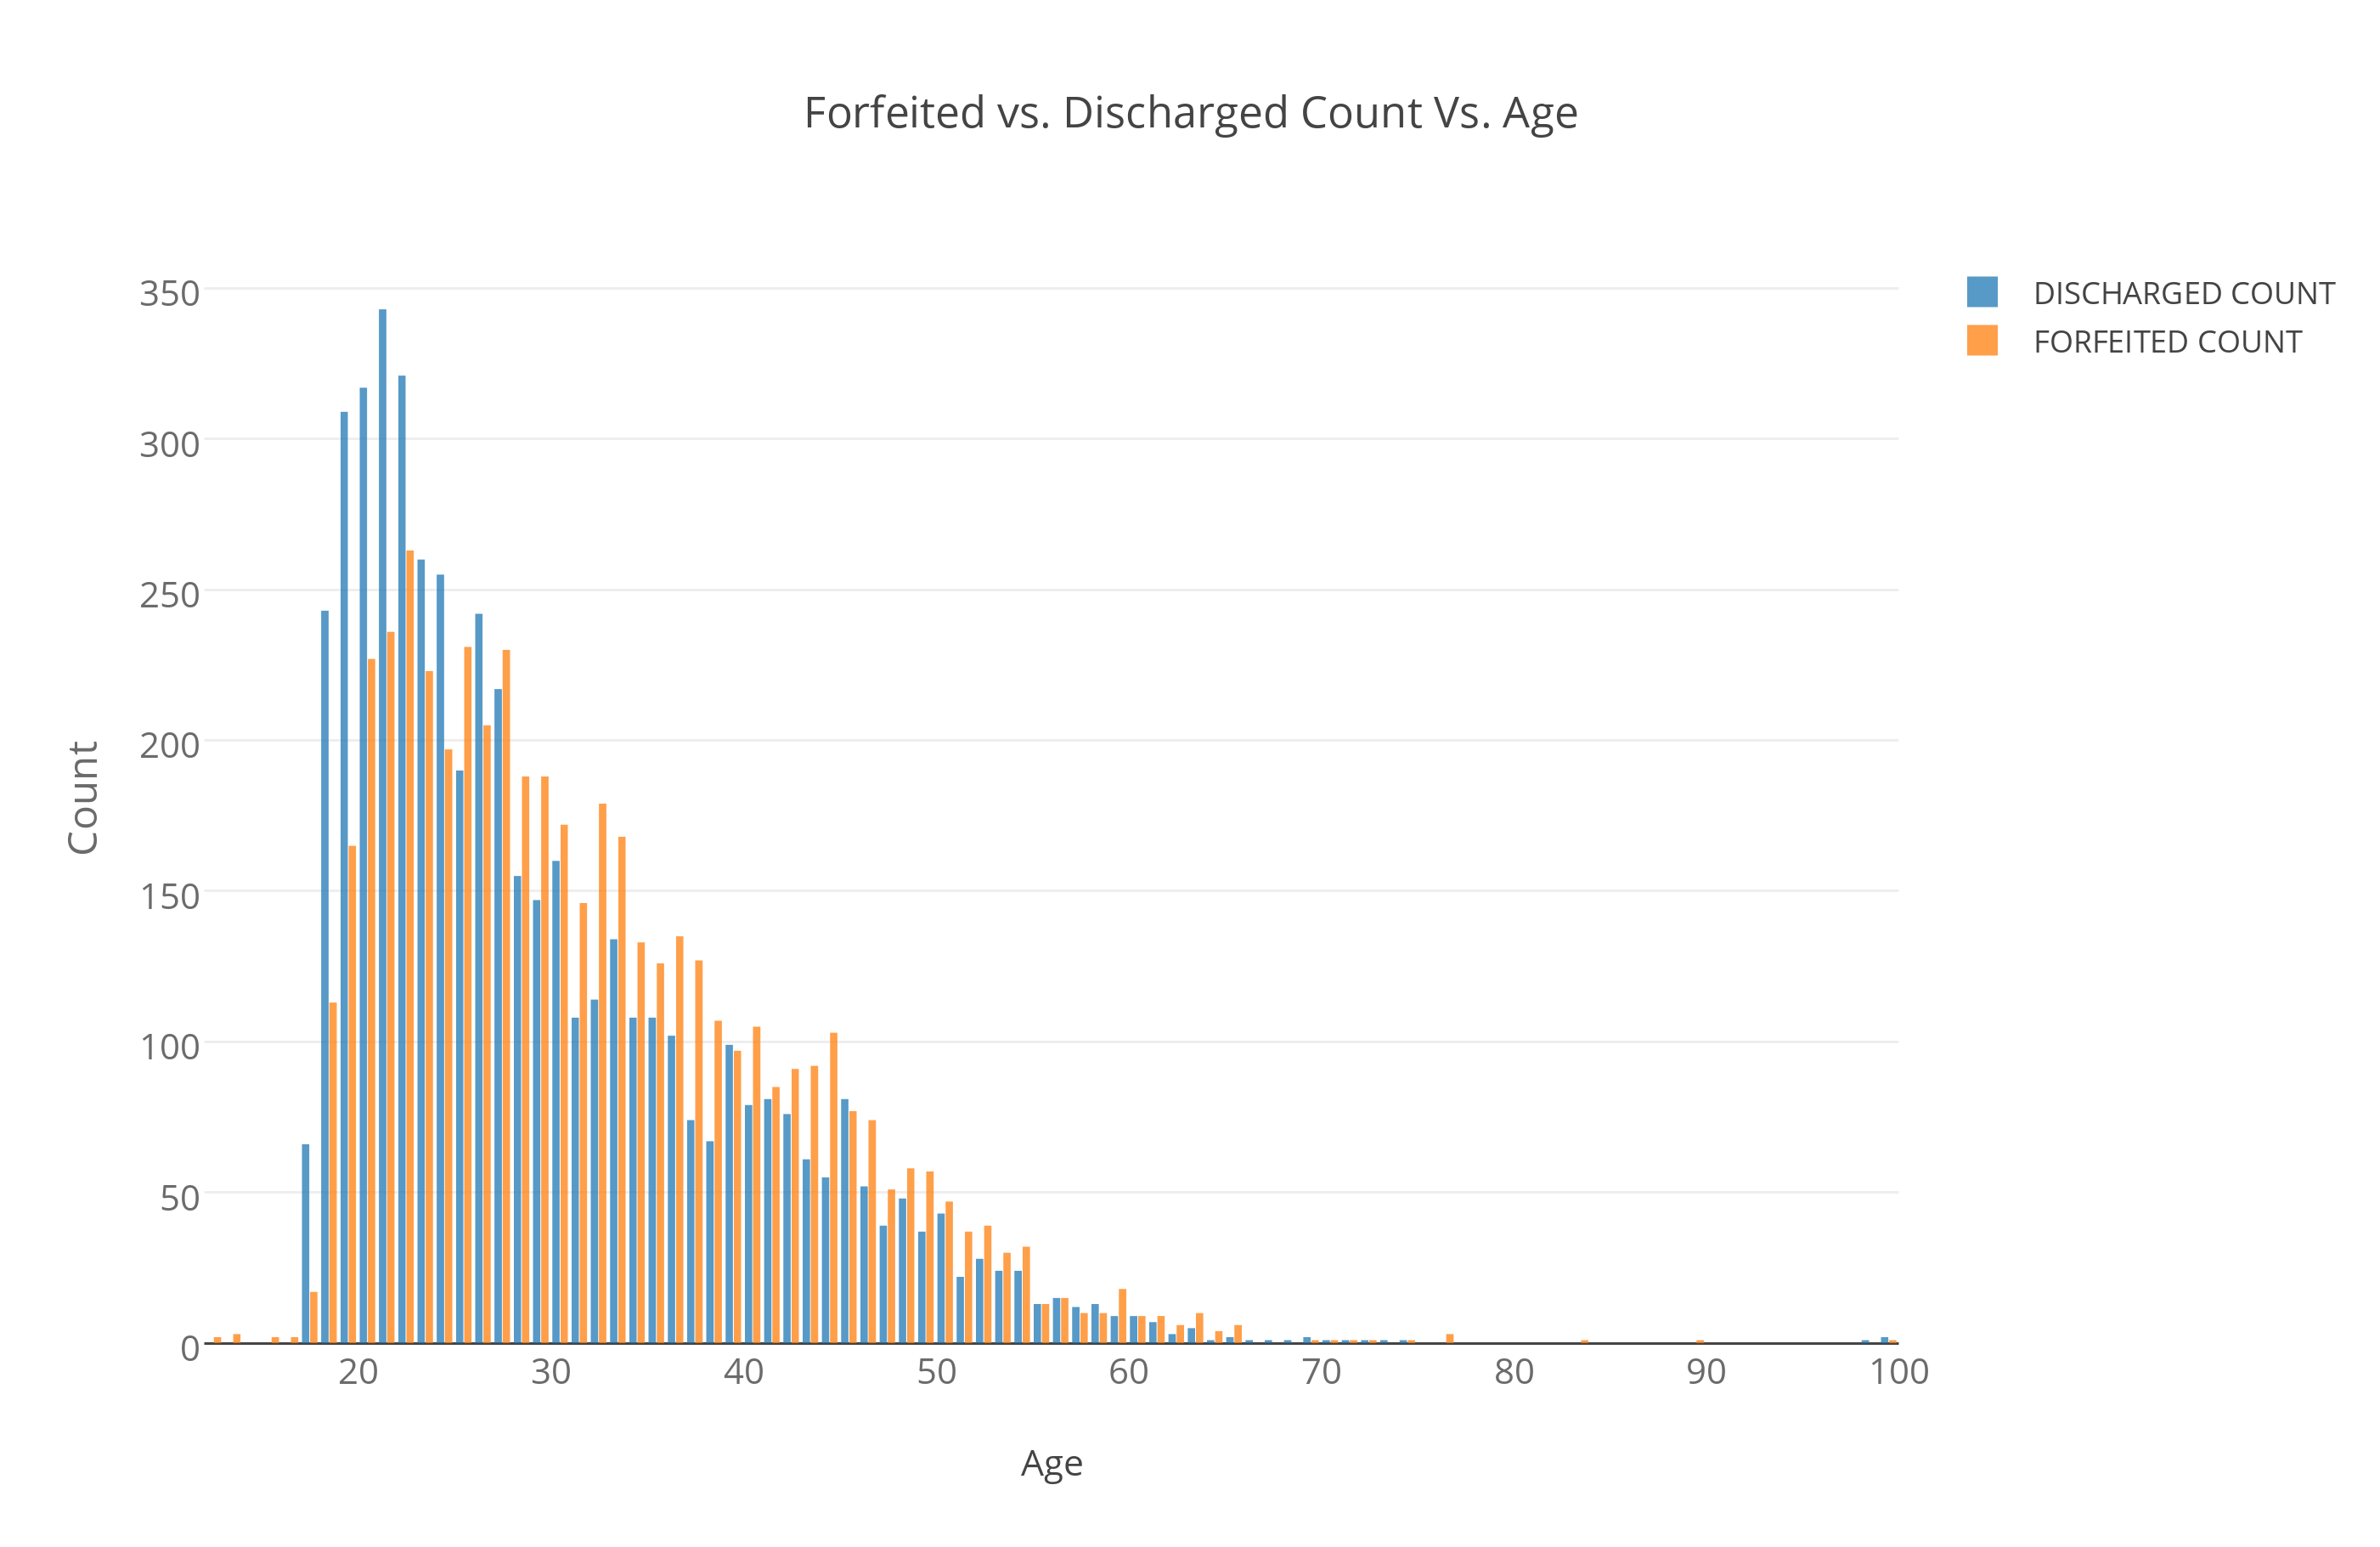
\includegraphics[width=0.5\paperwidth]{Forfeited_vs_Discharged_Count_Vs_Age.png}
\end{figure}

\item Gender
\end{enumerate}
~\\
\textbf{Characteristic of the environment:}
~\\
\begin{enumerate}
\setcounter{enumi}{2}
\item zipcode $\rightarrow$ income
\begin{figure}[H]
\centering
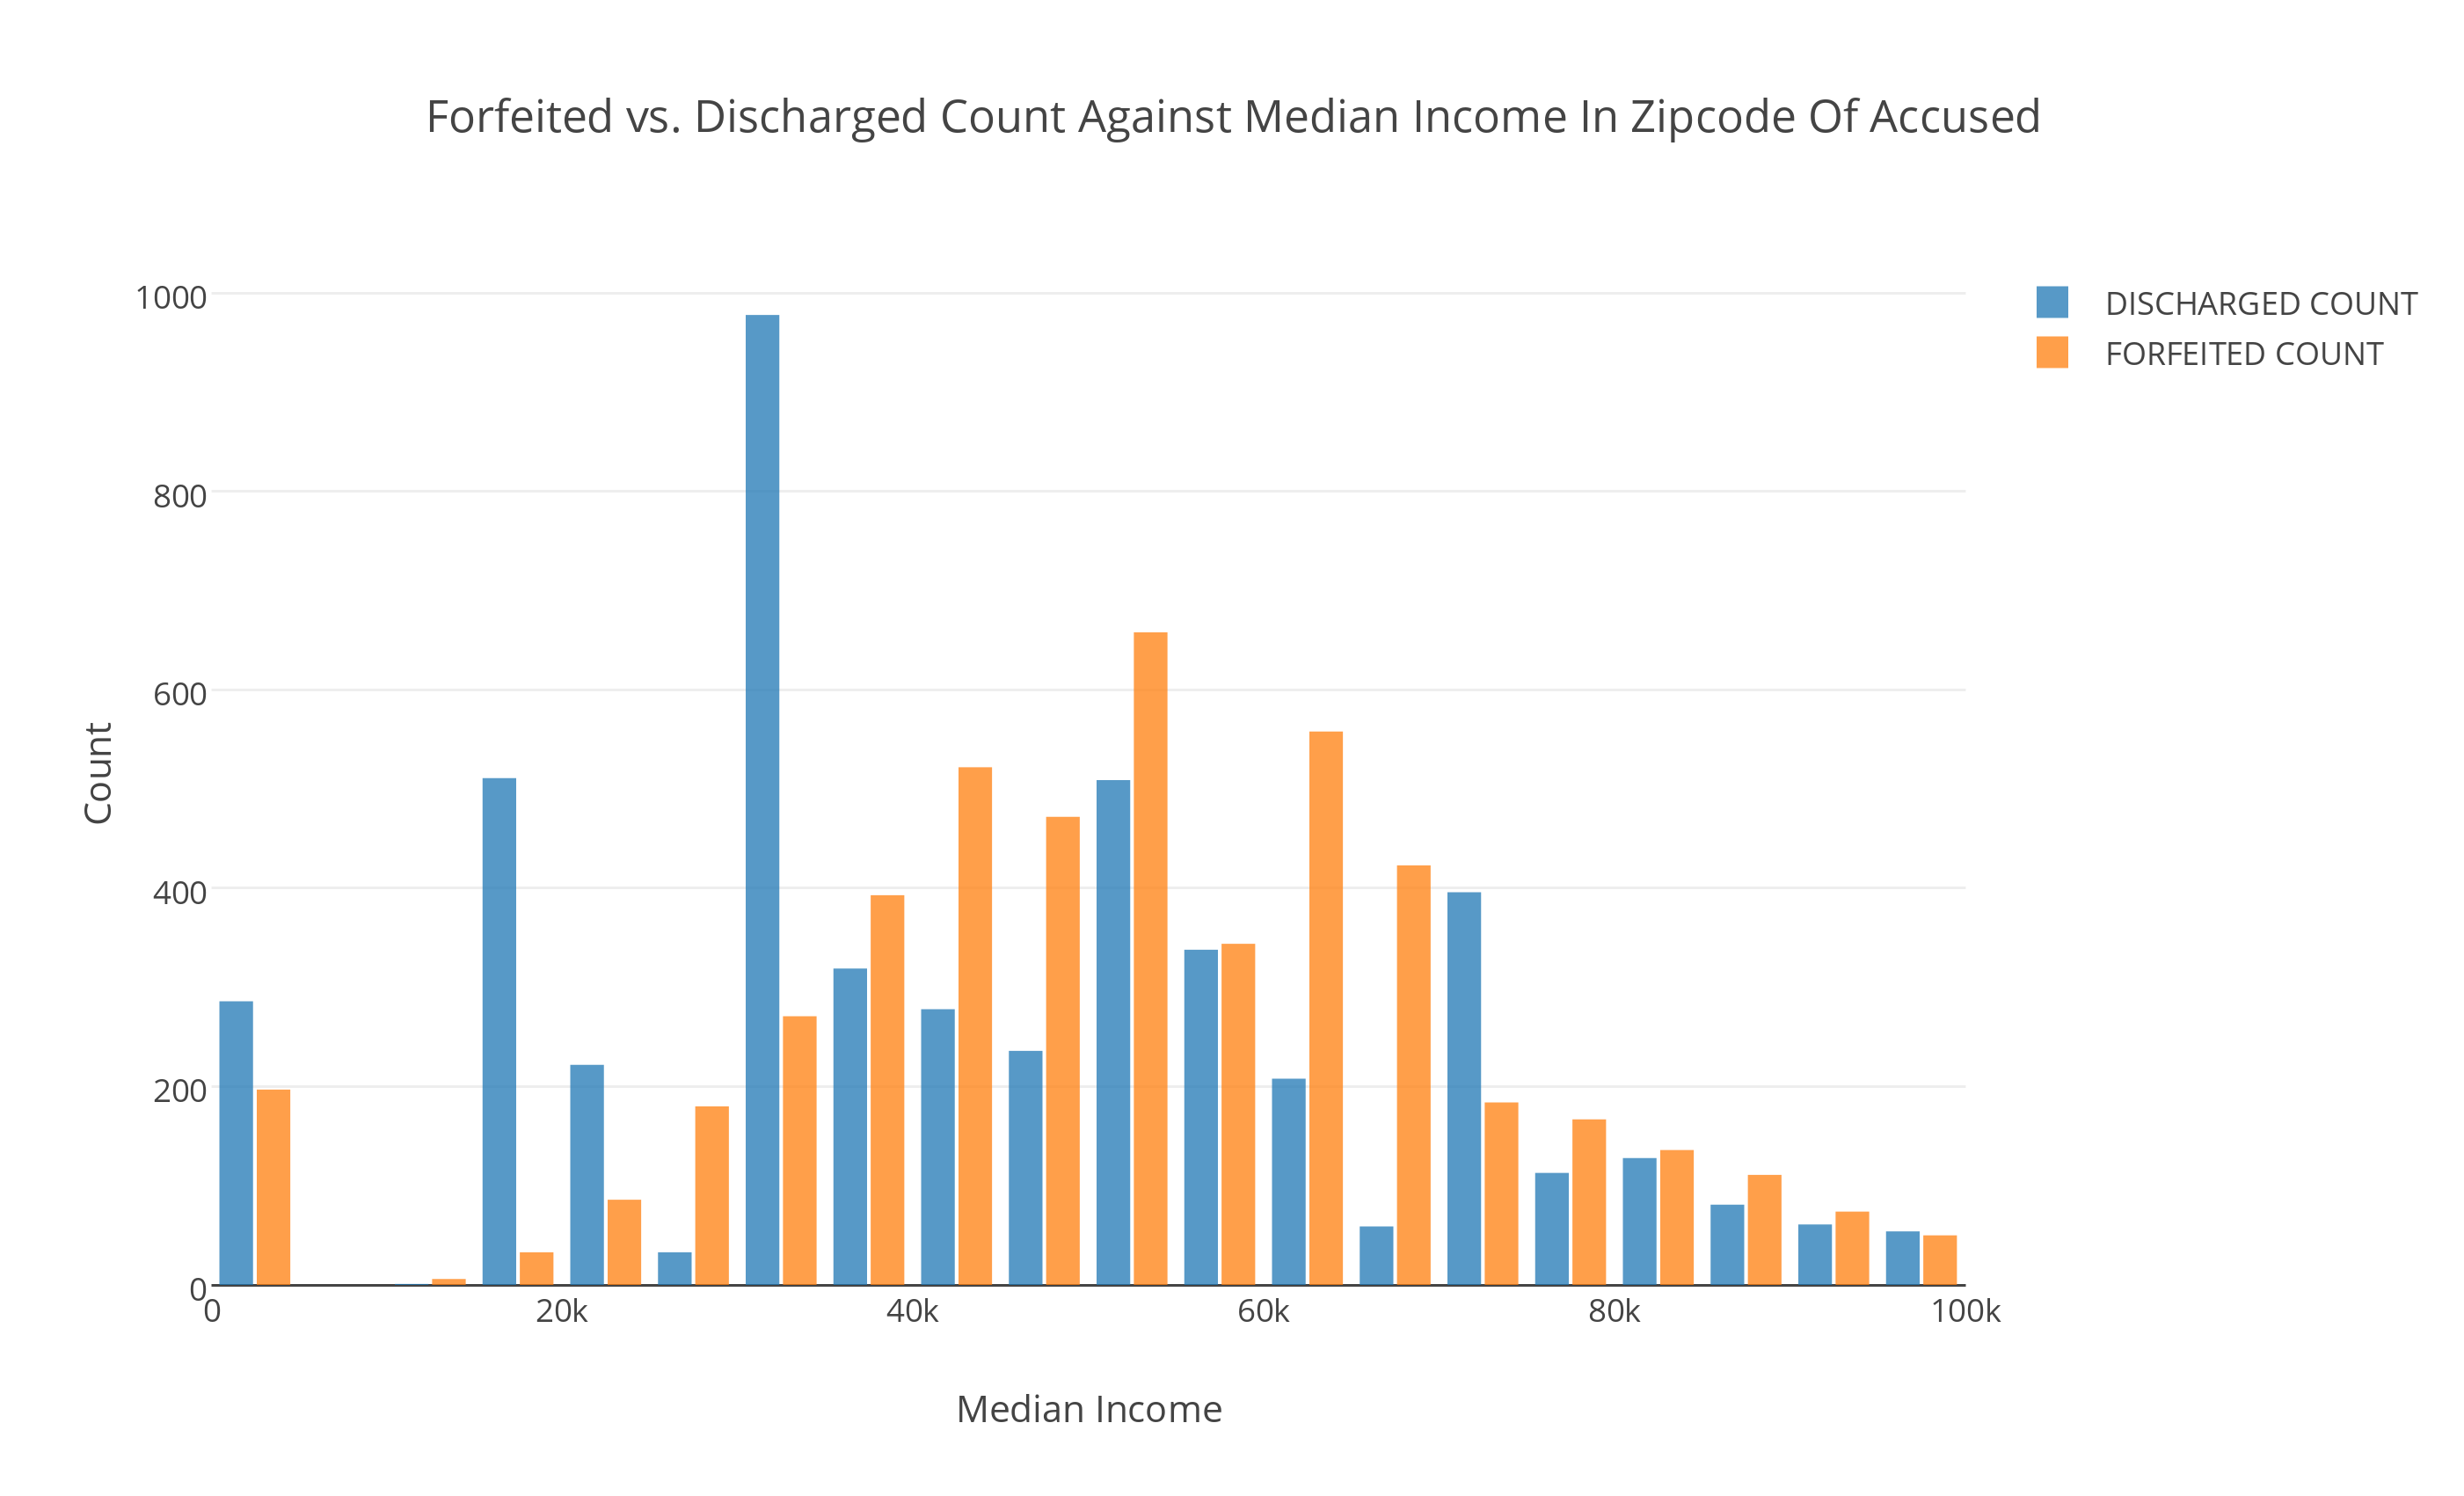
\includegraphics[width=0.5\paperwidth]{Forfeited_vs_Discharged_Count_Against_Median_Income_In_Zipcode_Of_Accused.png}
\end{figure}

The average income for a zipcode was obtained through an api to the latest available U.S. Census.   
\end{enumerate}
\textbf{Characteristic of the bond:}
~\\
\begin{enumerate}
\setcounter{enumi}{3}
\item Bond Amount
\begin{figure}[H]
\centering
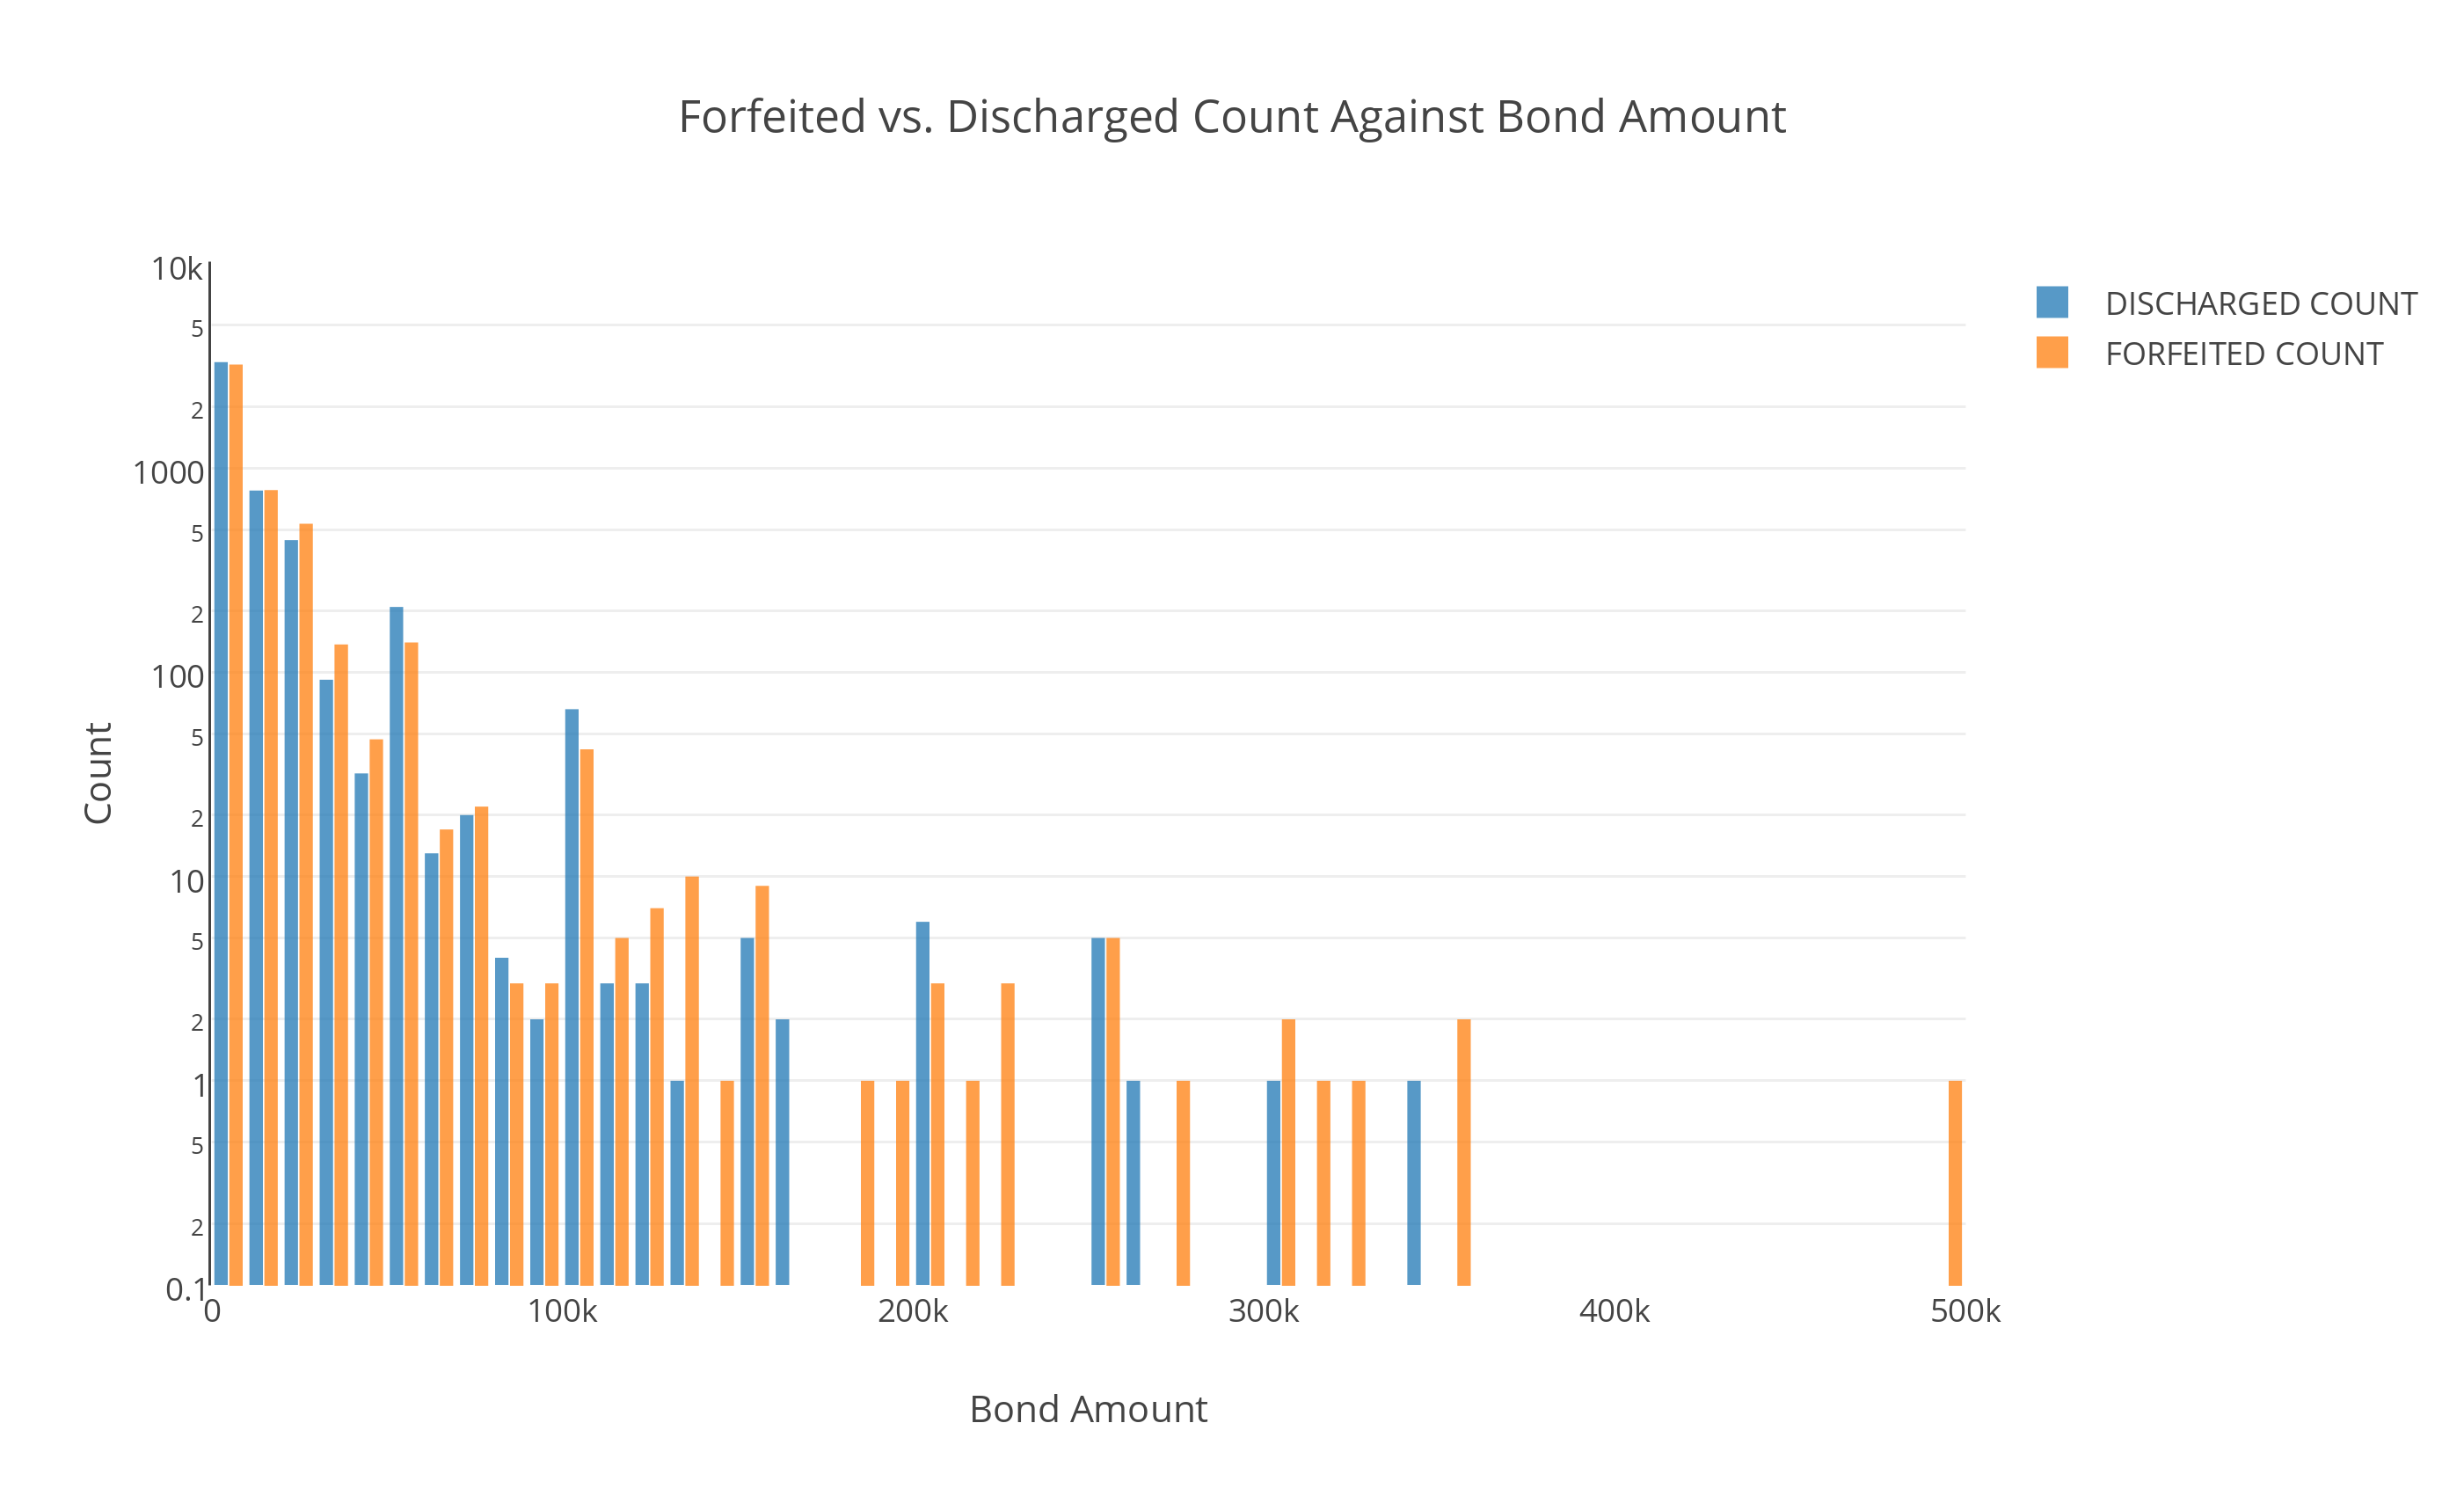
\includegraphics[width=0.5\paperwidth]{Forfeited_vs_Discharged_Count_Against_Bond_Amount.png}
\end{figure}
\end{enumerate}

\subsubsection{Validity of model}

A regression model: A statistical analysis used to predict scores on an outcome
variable based on scores on one or more predictor variables.\\
~\\
Can be as simple as:
\begin{equation}
Y = B_{0} + B_{1}X_{1} + B_{2}X_{2} + \ldots + \epsilon \\
\end{equation}
\begin{itemize}
\item Y: outcome variable (ex: Will fail to appear?)
\item X: pridictor variables (ex: Defendents age, bail amount \ldots)
\item B: coeffecients relating X's and Y
\item $\epsilon$: error terms (a.k.a residual)
\end{itemize}
~\\
Finding a relationship between X and Y which minimizes the model errors gives us:

\begin{center}
\begin{verbatim}
Deviance Residuals: 
    Min       1Q   Median       3Q      Max  
-2.3472  -1.0933  -0.7349   1.1296   1.8166  

Coefficients:
                Estimate Std. Error z value Pr(>|z|)    
(Intercept)    -1.835339   0.099919 -18.368  < 2e-16 ***
catBond_Amount  0.013388   0.006470   2.069  0.03854 *  
age             0.031466   0.002381  13.213  < 2e-16 ***
catZipIncome    0.183926   0.010761  17.092  < 2e-16 ***
genderM        -0.166691   0.053297  -3.128  0.00176 ** 
---
Signif. codes:  0 ‘***’ 0.001 ‘**’ 0.01 ‘*’ 0.05 ‘.’ 0.1 ‘ ’ 1
\end{verbatim}
\end{center}

~\\
example model predicitions:
~\\
~\\
\underline{Defendent 1:}
~\\
\begin{itemize}
\item Age: 38
\item Gender: Female 
\item Bond Amount \$35,000
\item Zipcode Income  \$75,392
\end{itemize}
~\\
Probablity calculated by the model: 75\% to fail to appear
In reality, the bond was forfeited. This is called a ``true positive''.


~\\
\underline{Defendent 2:}
~\\
\begin{itemize}
\item Age:             23   
\item Gender:          Male
\item Bond Amount:    \$5,000
\item Zipcode Income: \$101,905
\end{itemize}

Probablity calculated by the model: 62\% to fail to appear
In reality, the defendant appeared in court and the bond was discharged. 
This is called a ``false positive''.

The aim is to maximize true positives and minimize false positives. 

\underline{Project Goal}

\begin{figure}[H]
\centering
%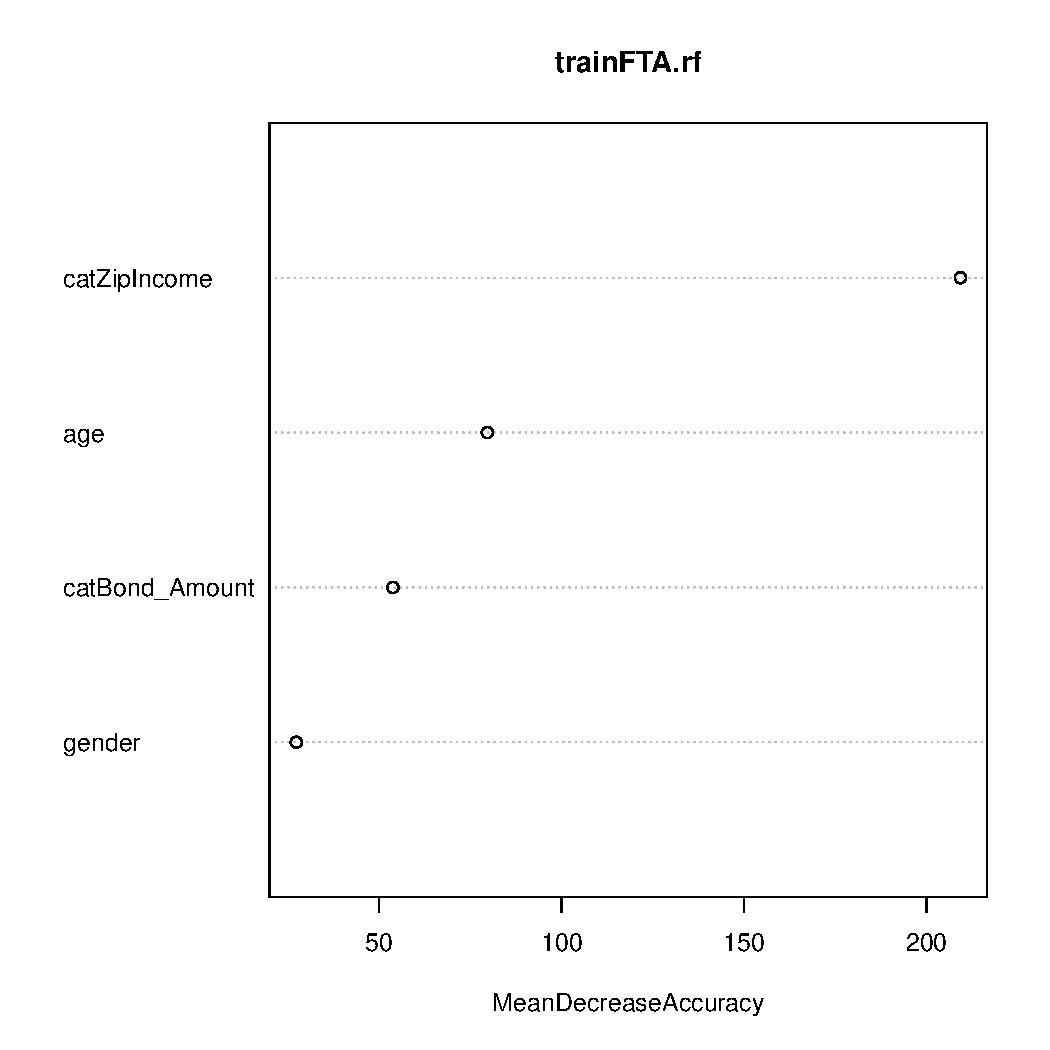
\includegraphics[width=0.45\paperwidth,page=1]{varPlot.pdf}
\includegraphics[width=0.45\paperwidth,page=3]{varPlot.pdf}
\end{figure}
 

\subsection{Project B: \underline{Reporting of agent performance}}

Build performance plots of agents and AIA. Reports could include three granularities, agent level, state level, and national level: 
\begin{itemize}
\item premiums and BUF amount obtained from agents. 
\item Total penal written by agent
\item granularity: agent, state, national
\item comparison of these values by date ranges
\end{itemize}

%\begin{figure}[b]
%\centering
%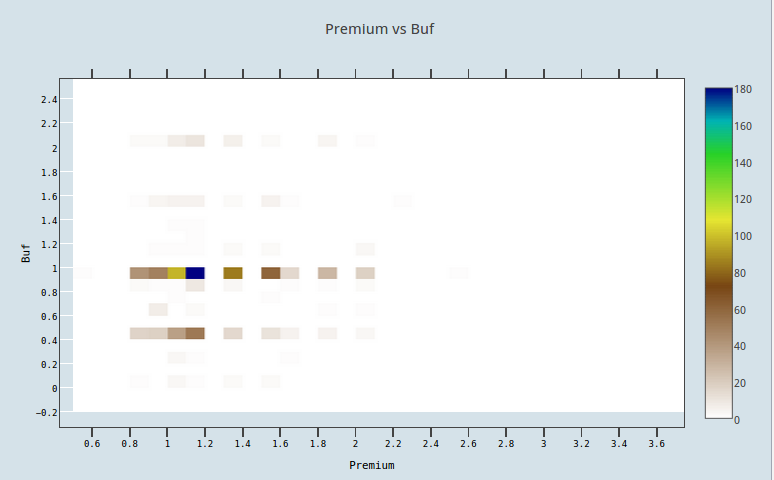
\includegraphics[width=0.45\paperwidth]{bufVsPrem2.png}
%\end{figure}

\begin{figure}[H]
\centering
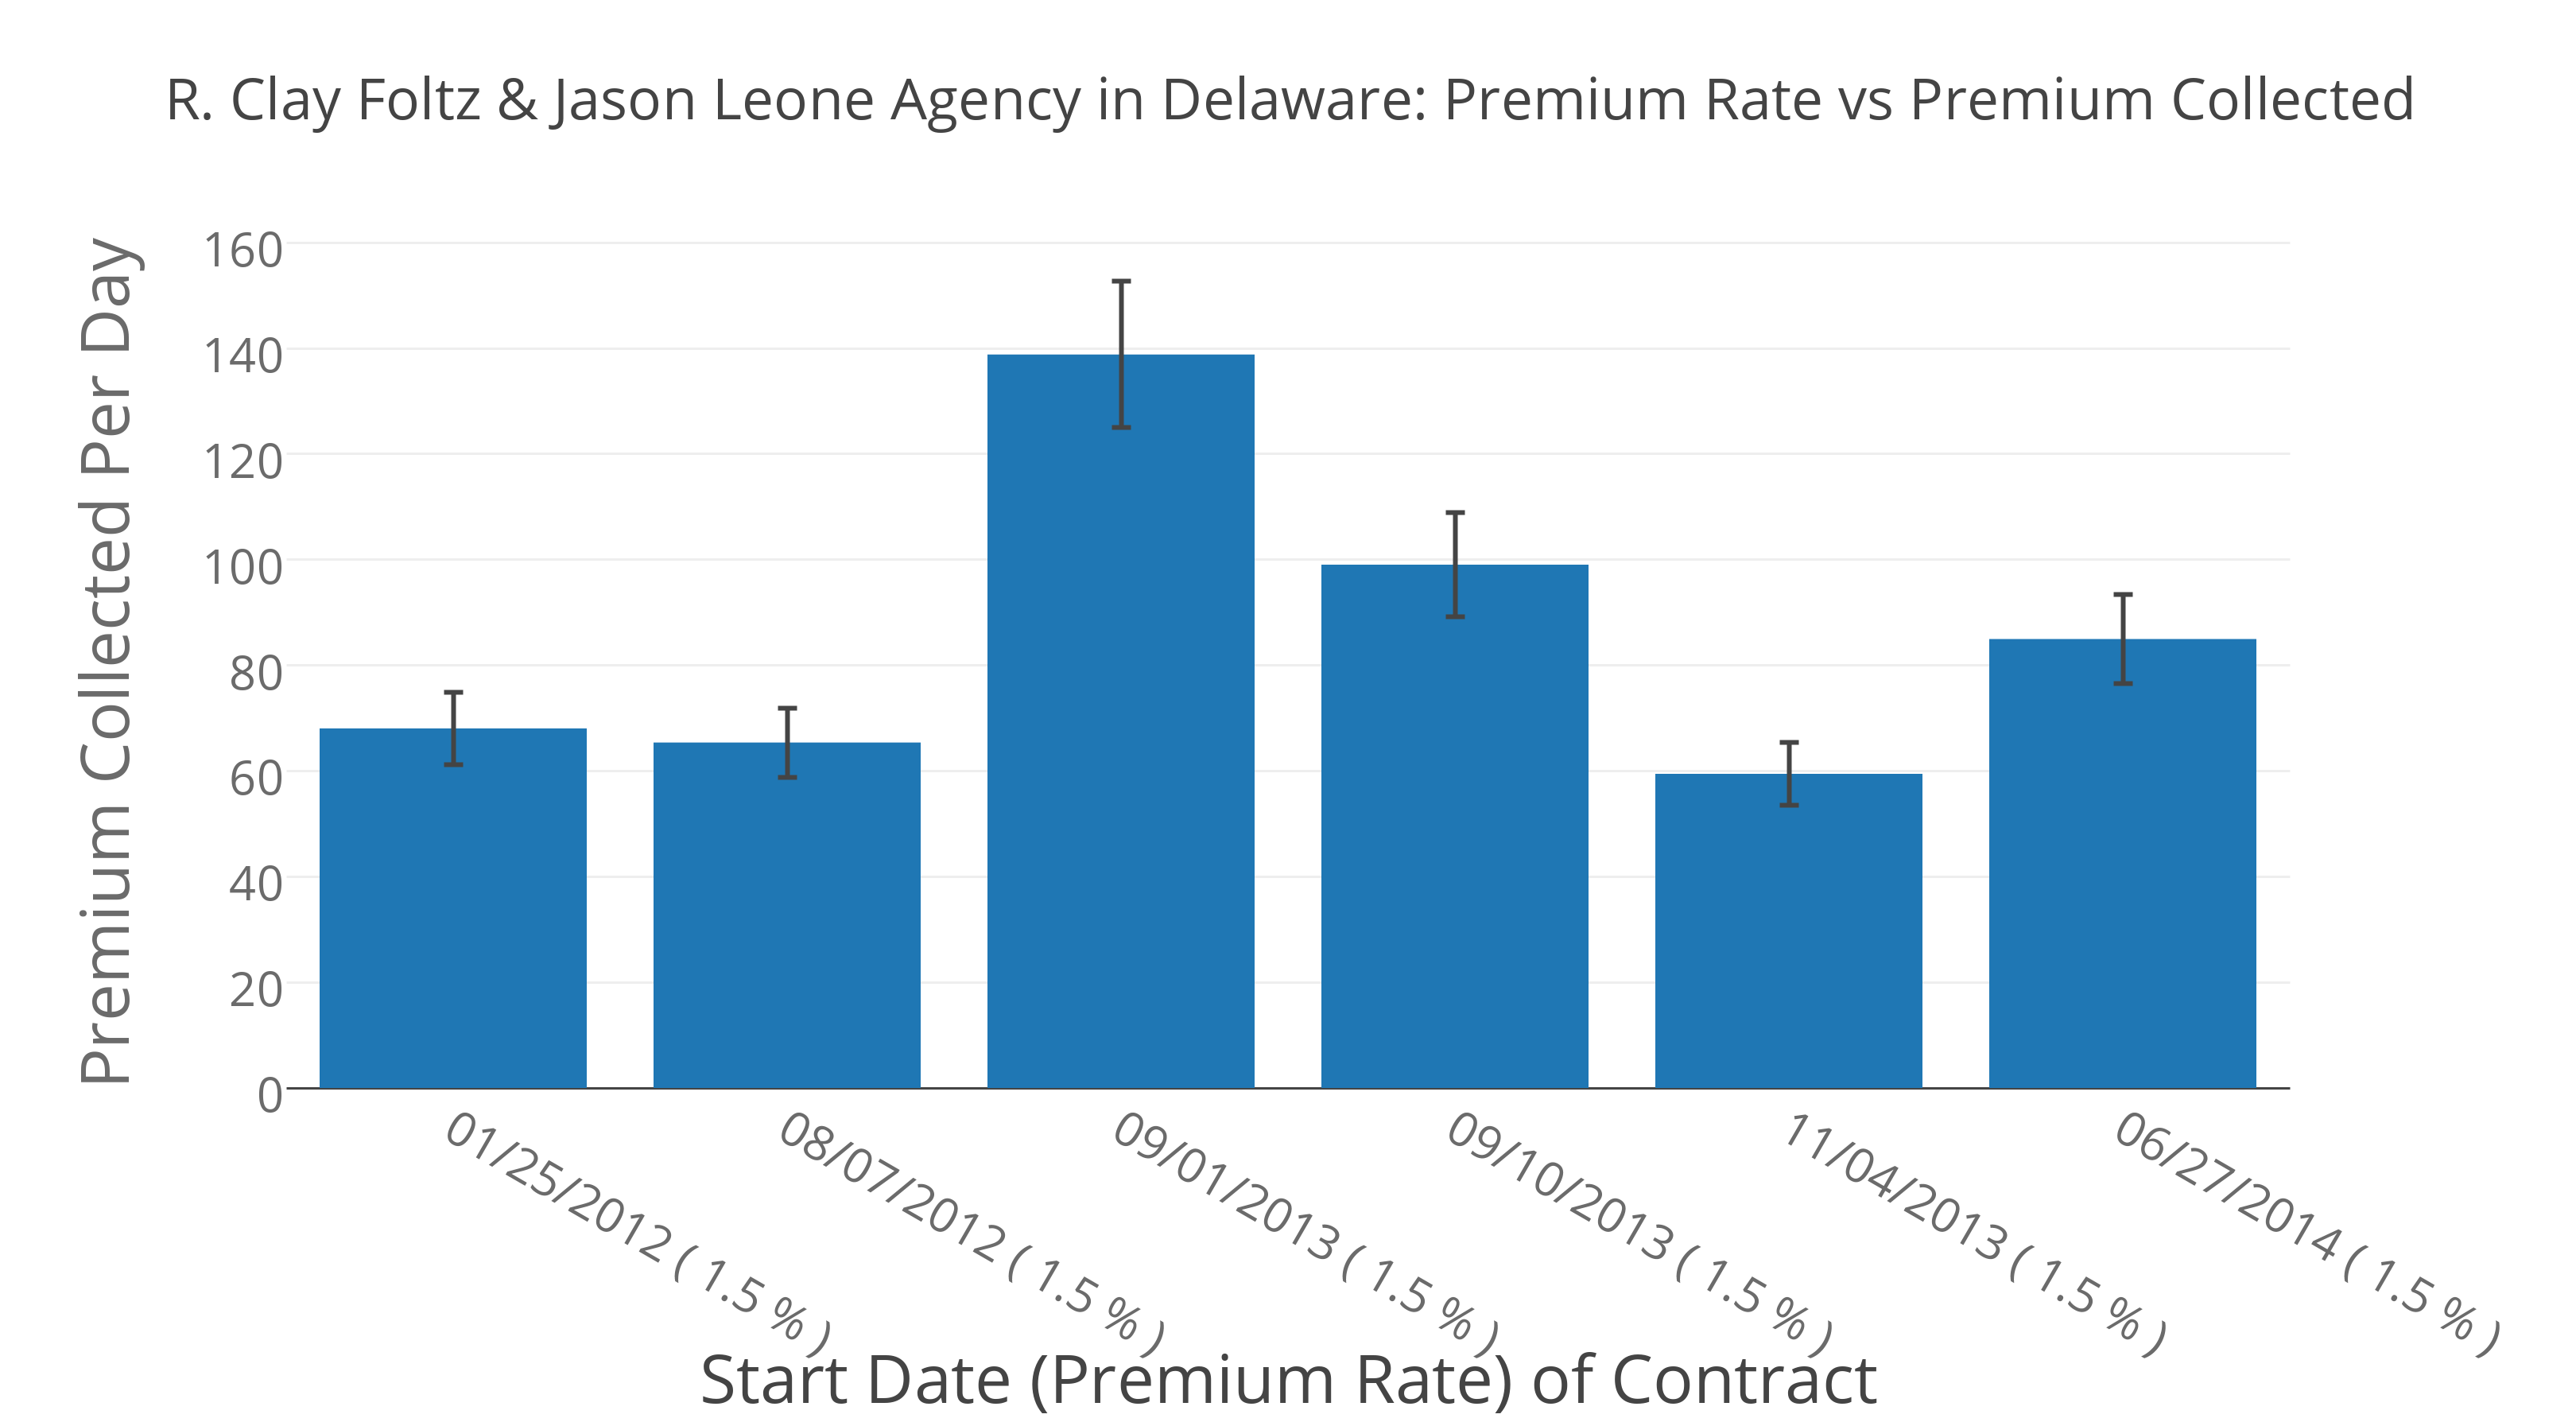
\includegraphics[width=0.34\paperwidth]{R_Clay_Foltz_&_Jason_Leone_Agency_in_Delaware-_Premium_Rate_vs_Premium_Collected.png}\\
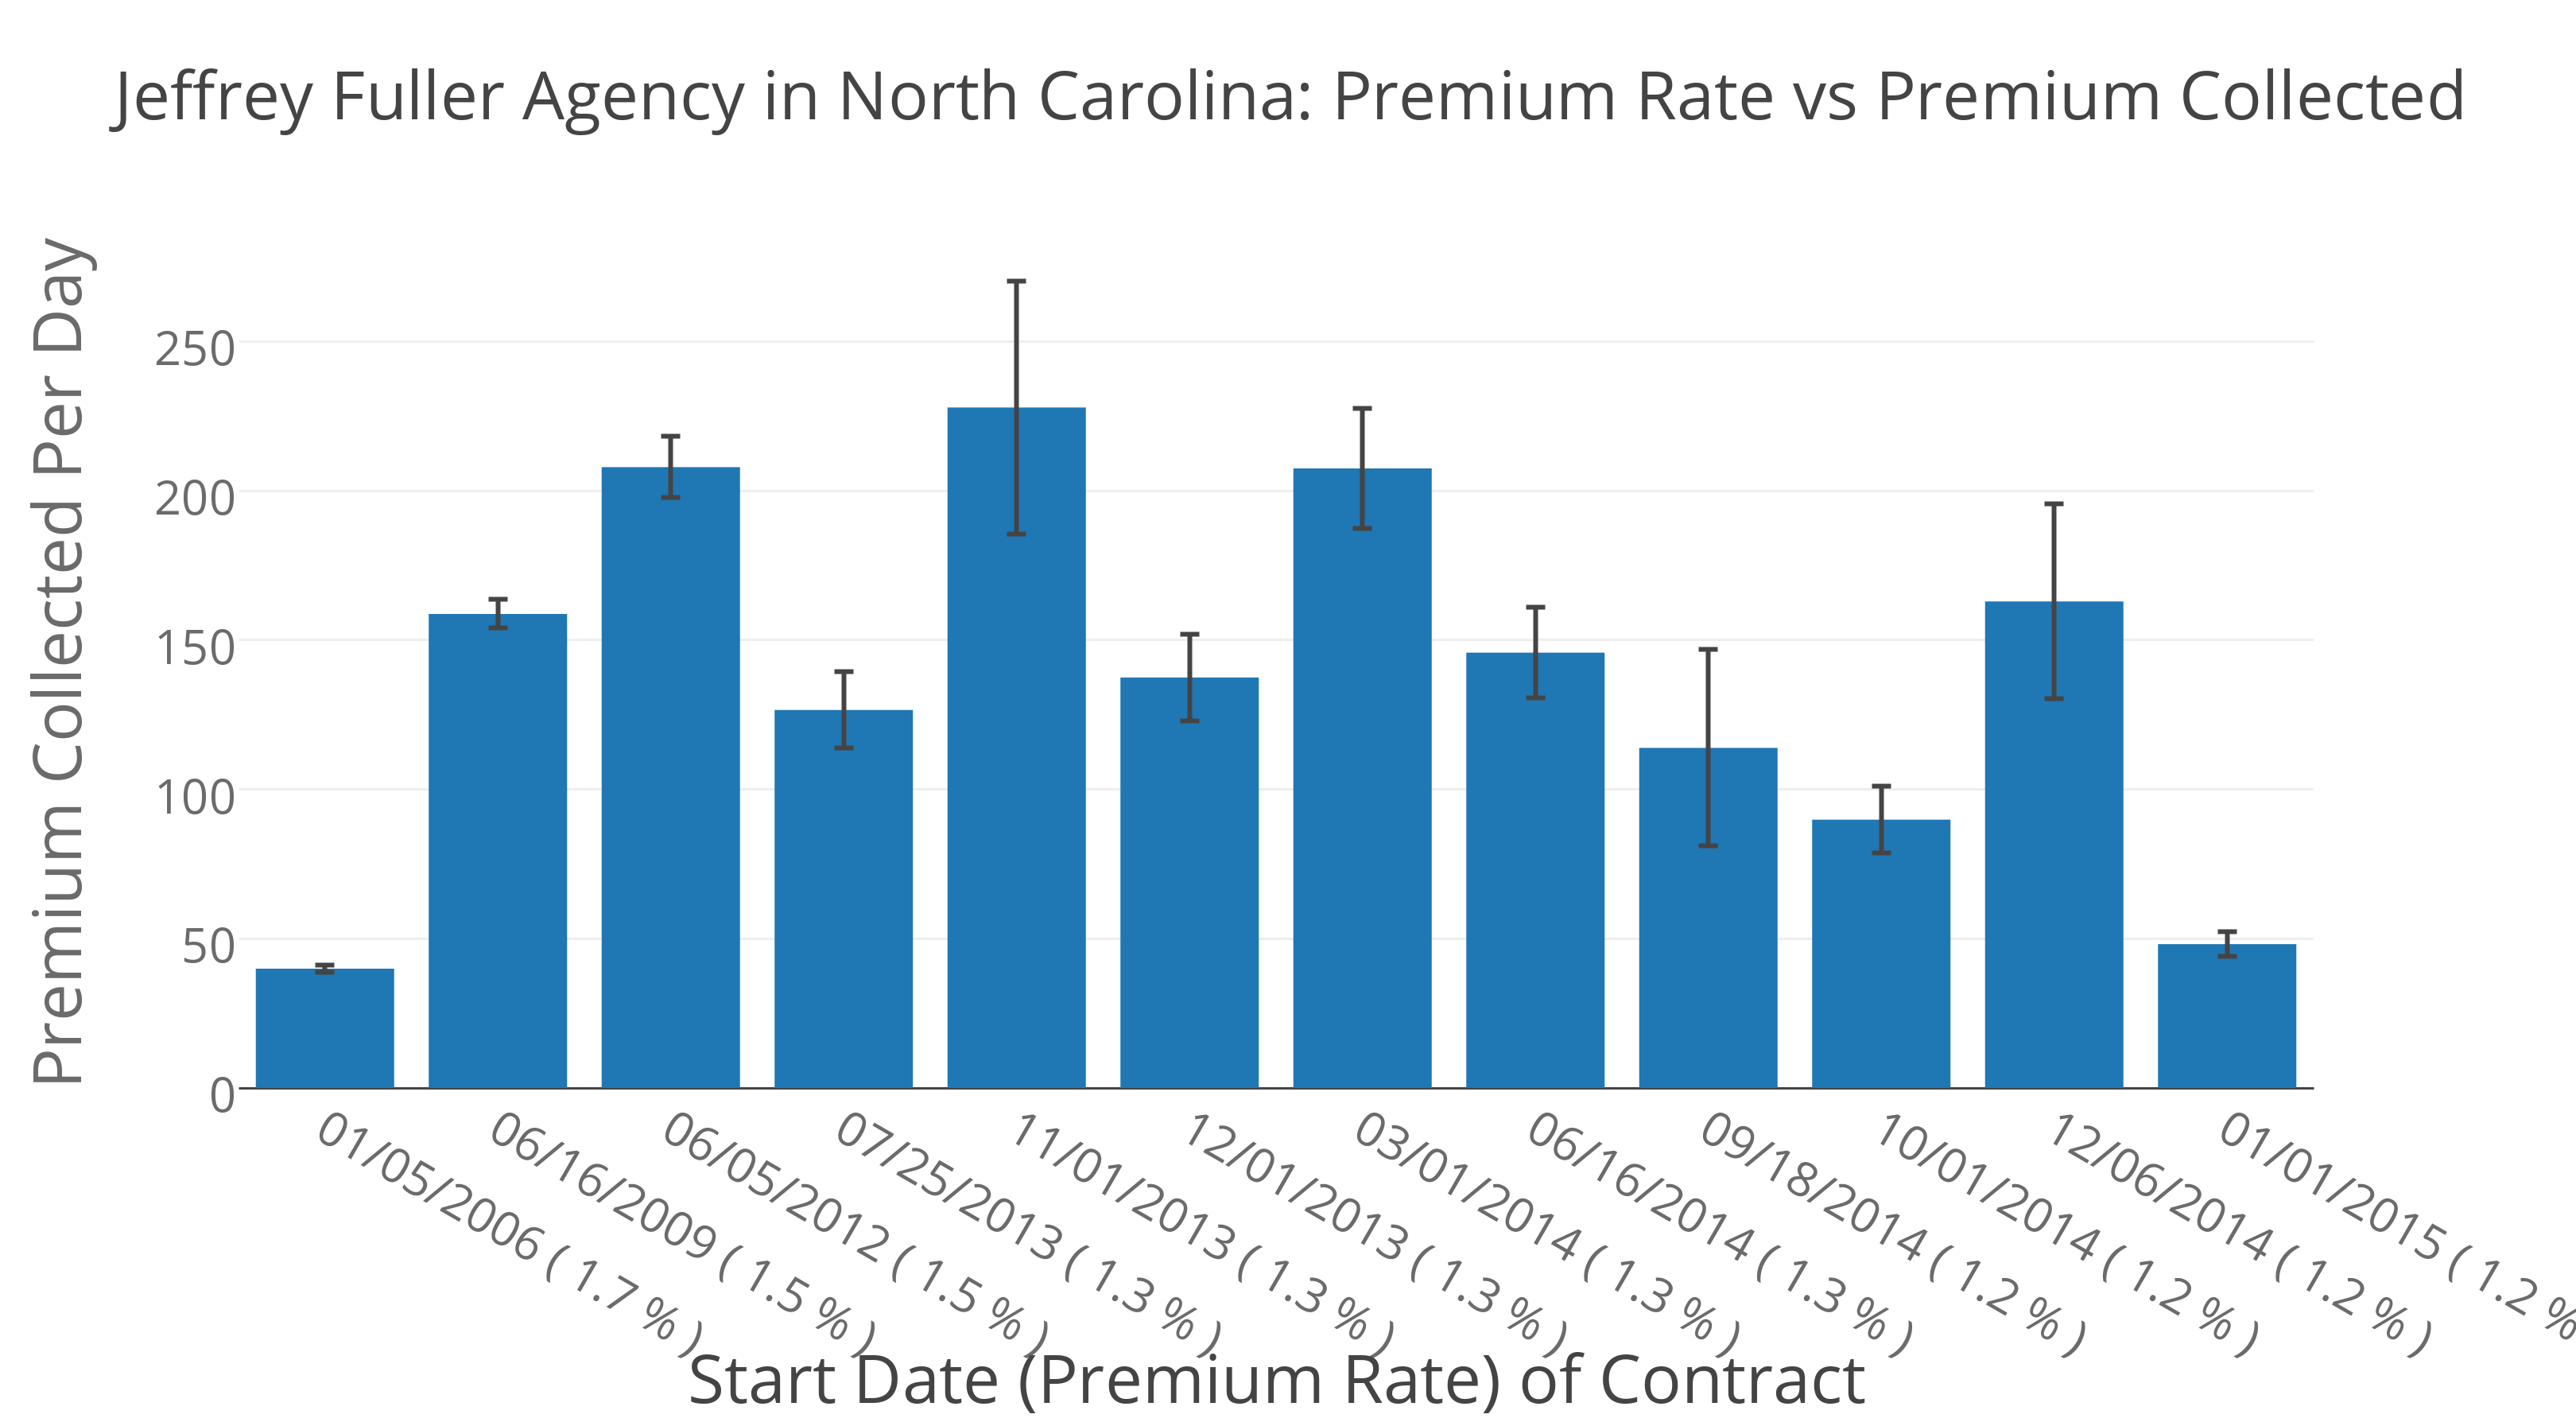
\includegraphics[width=0.34\paperwidth]{Jeffrey_Fuller_Agency_in_North_Carolina-_Premium_Rate_vs_Premium_Collected.png}
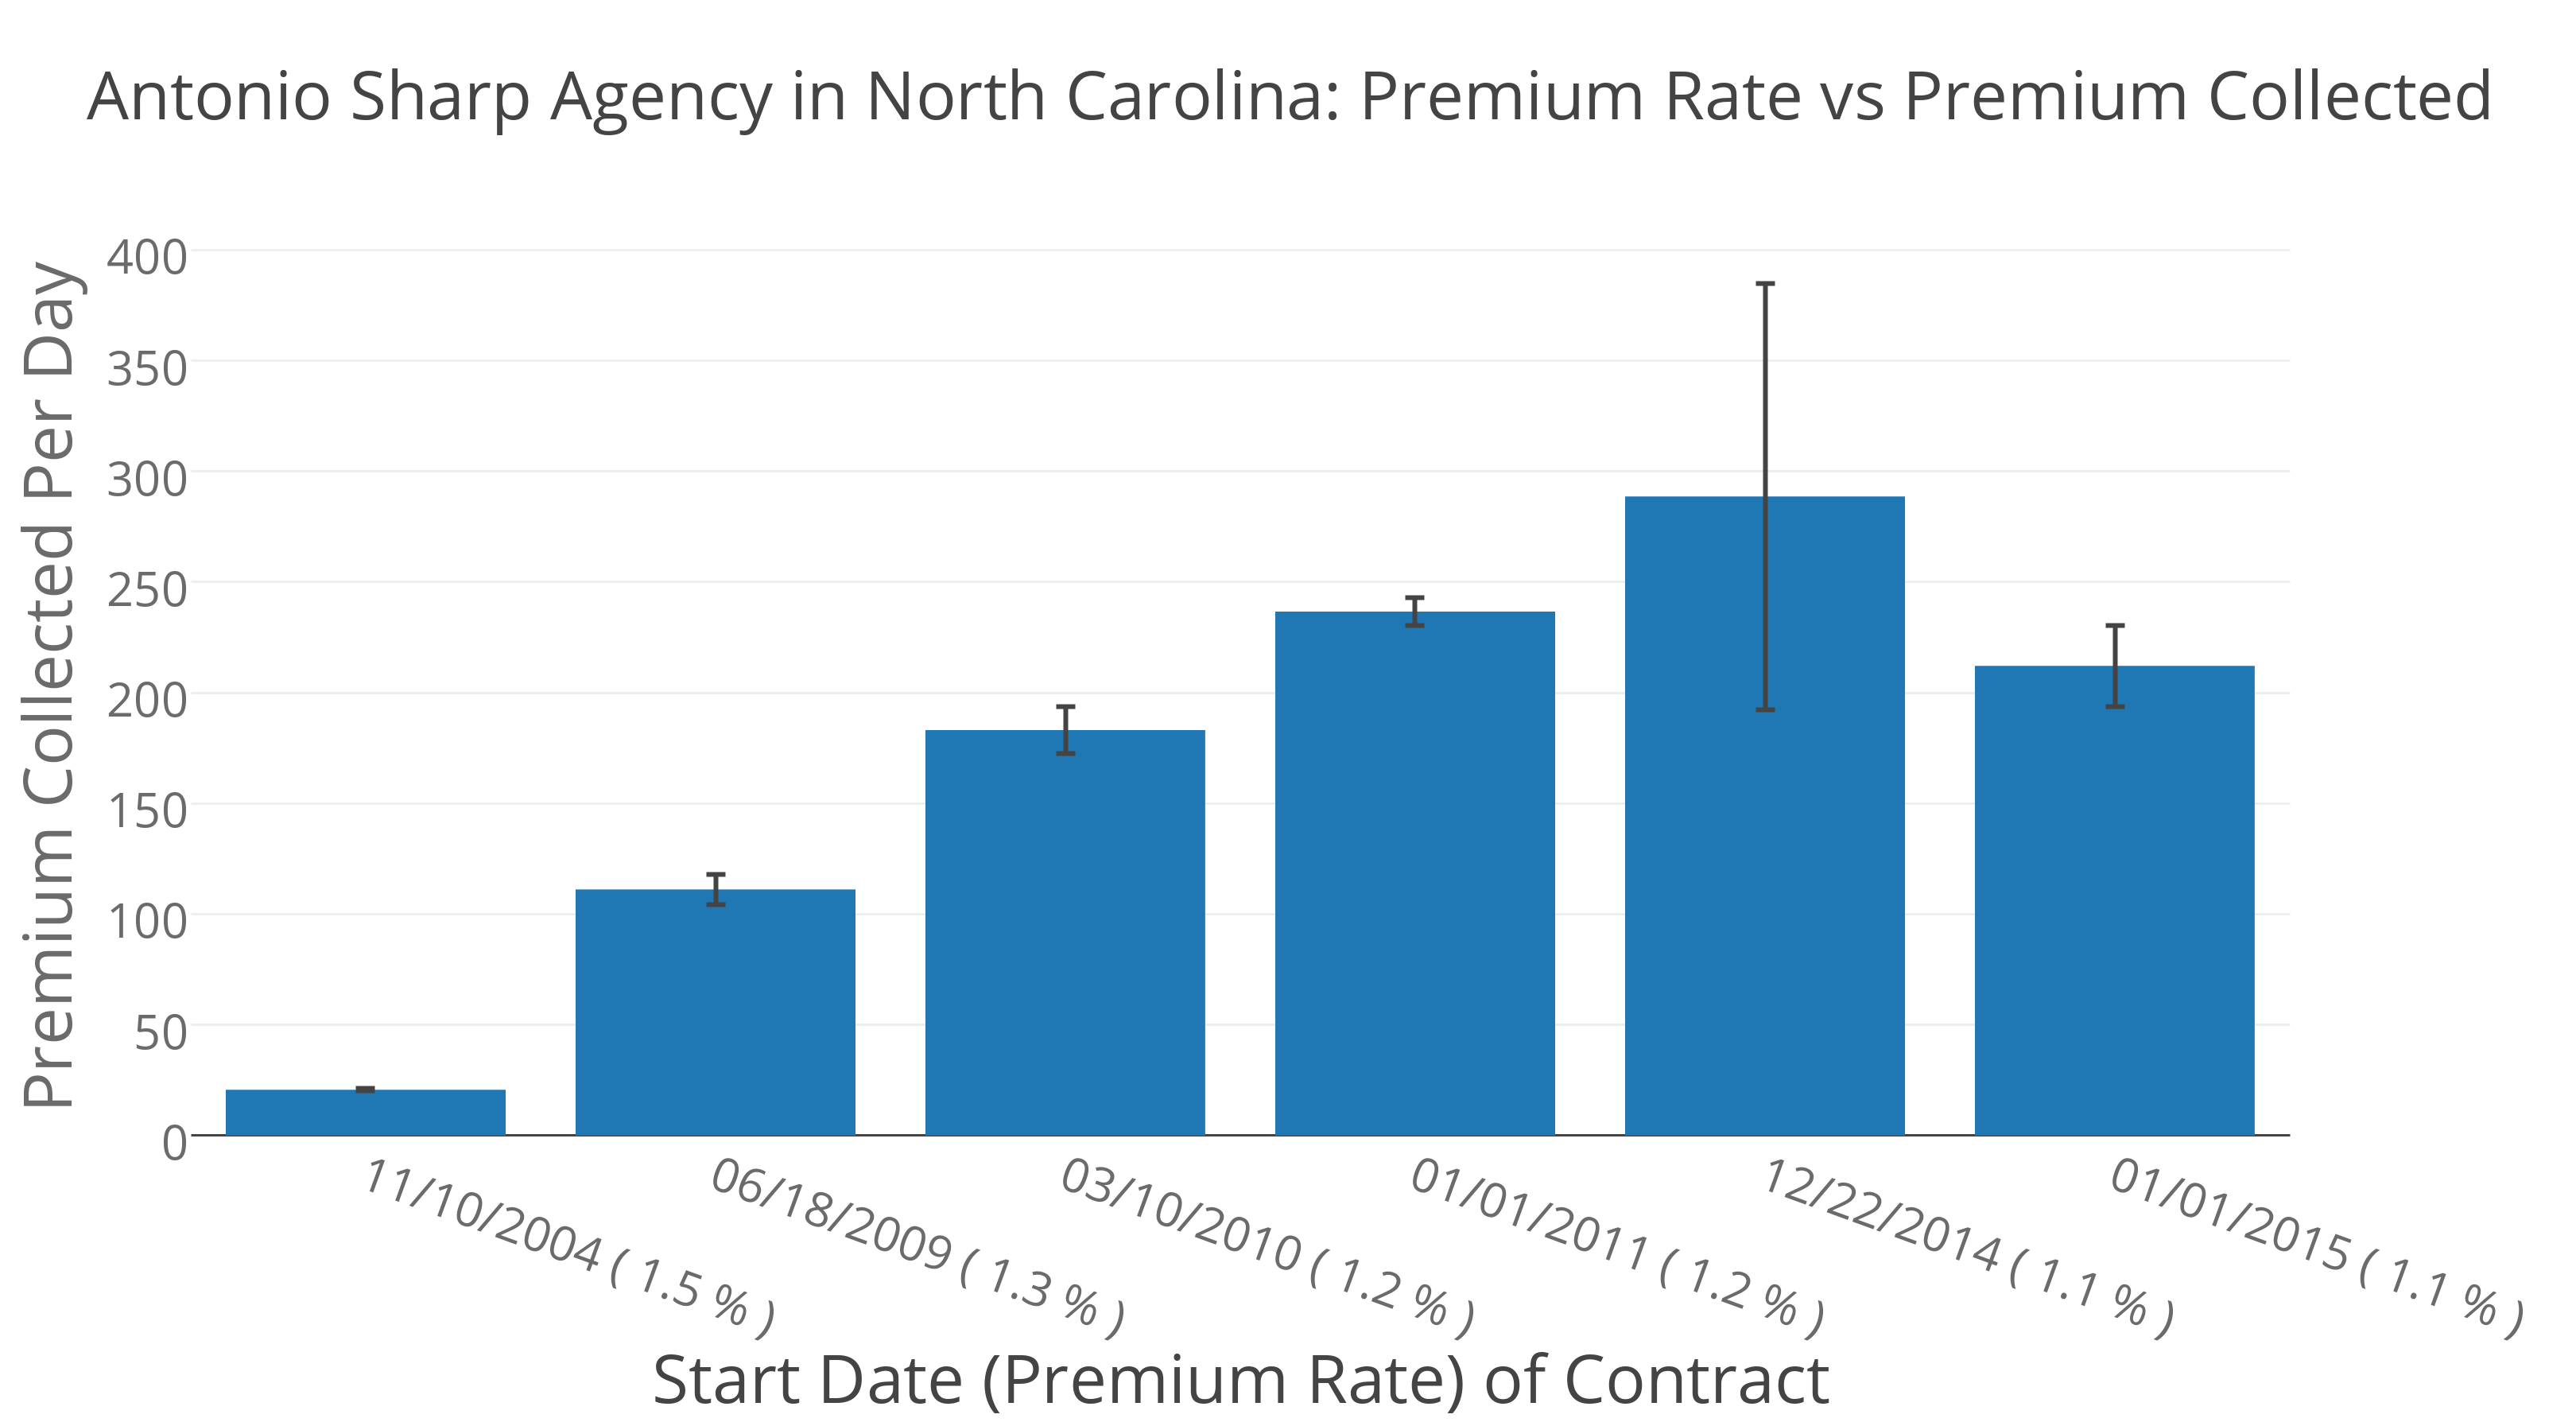
\includegraphics[width=0.34\paperwidth]{Antonio_Sharp_Agency_in_North_Carolina-_Premium_Rate_vs_Premium_Collected.png}
\end{figure}
\begin{figure}[H]
\centering
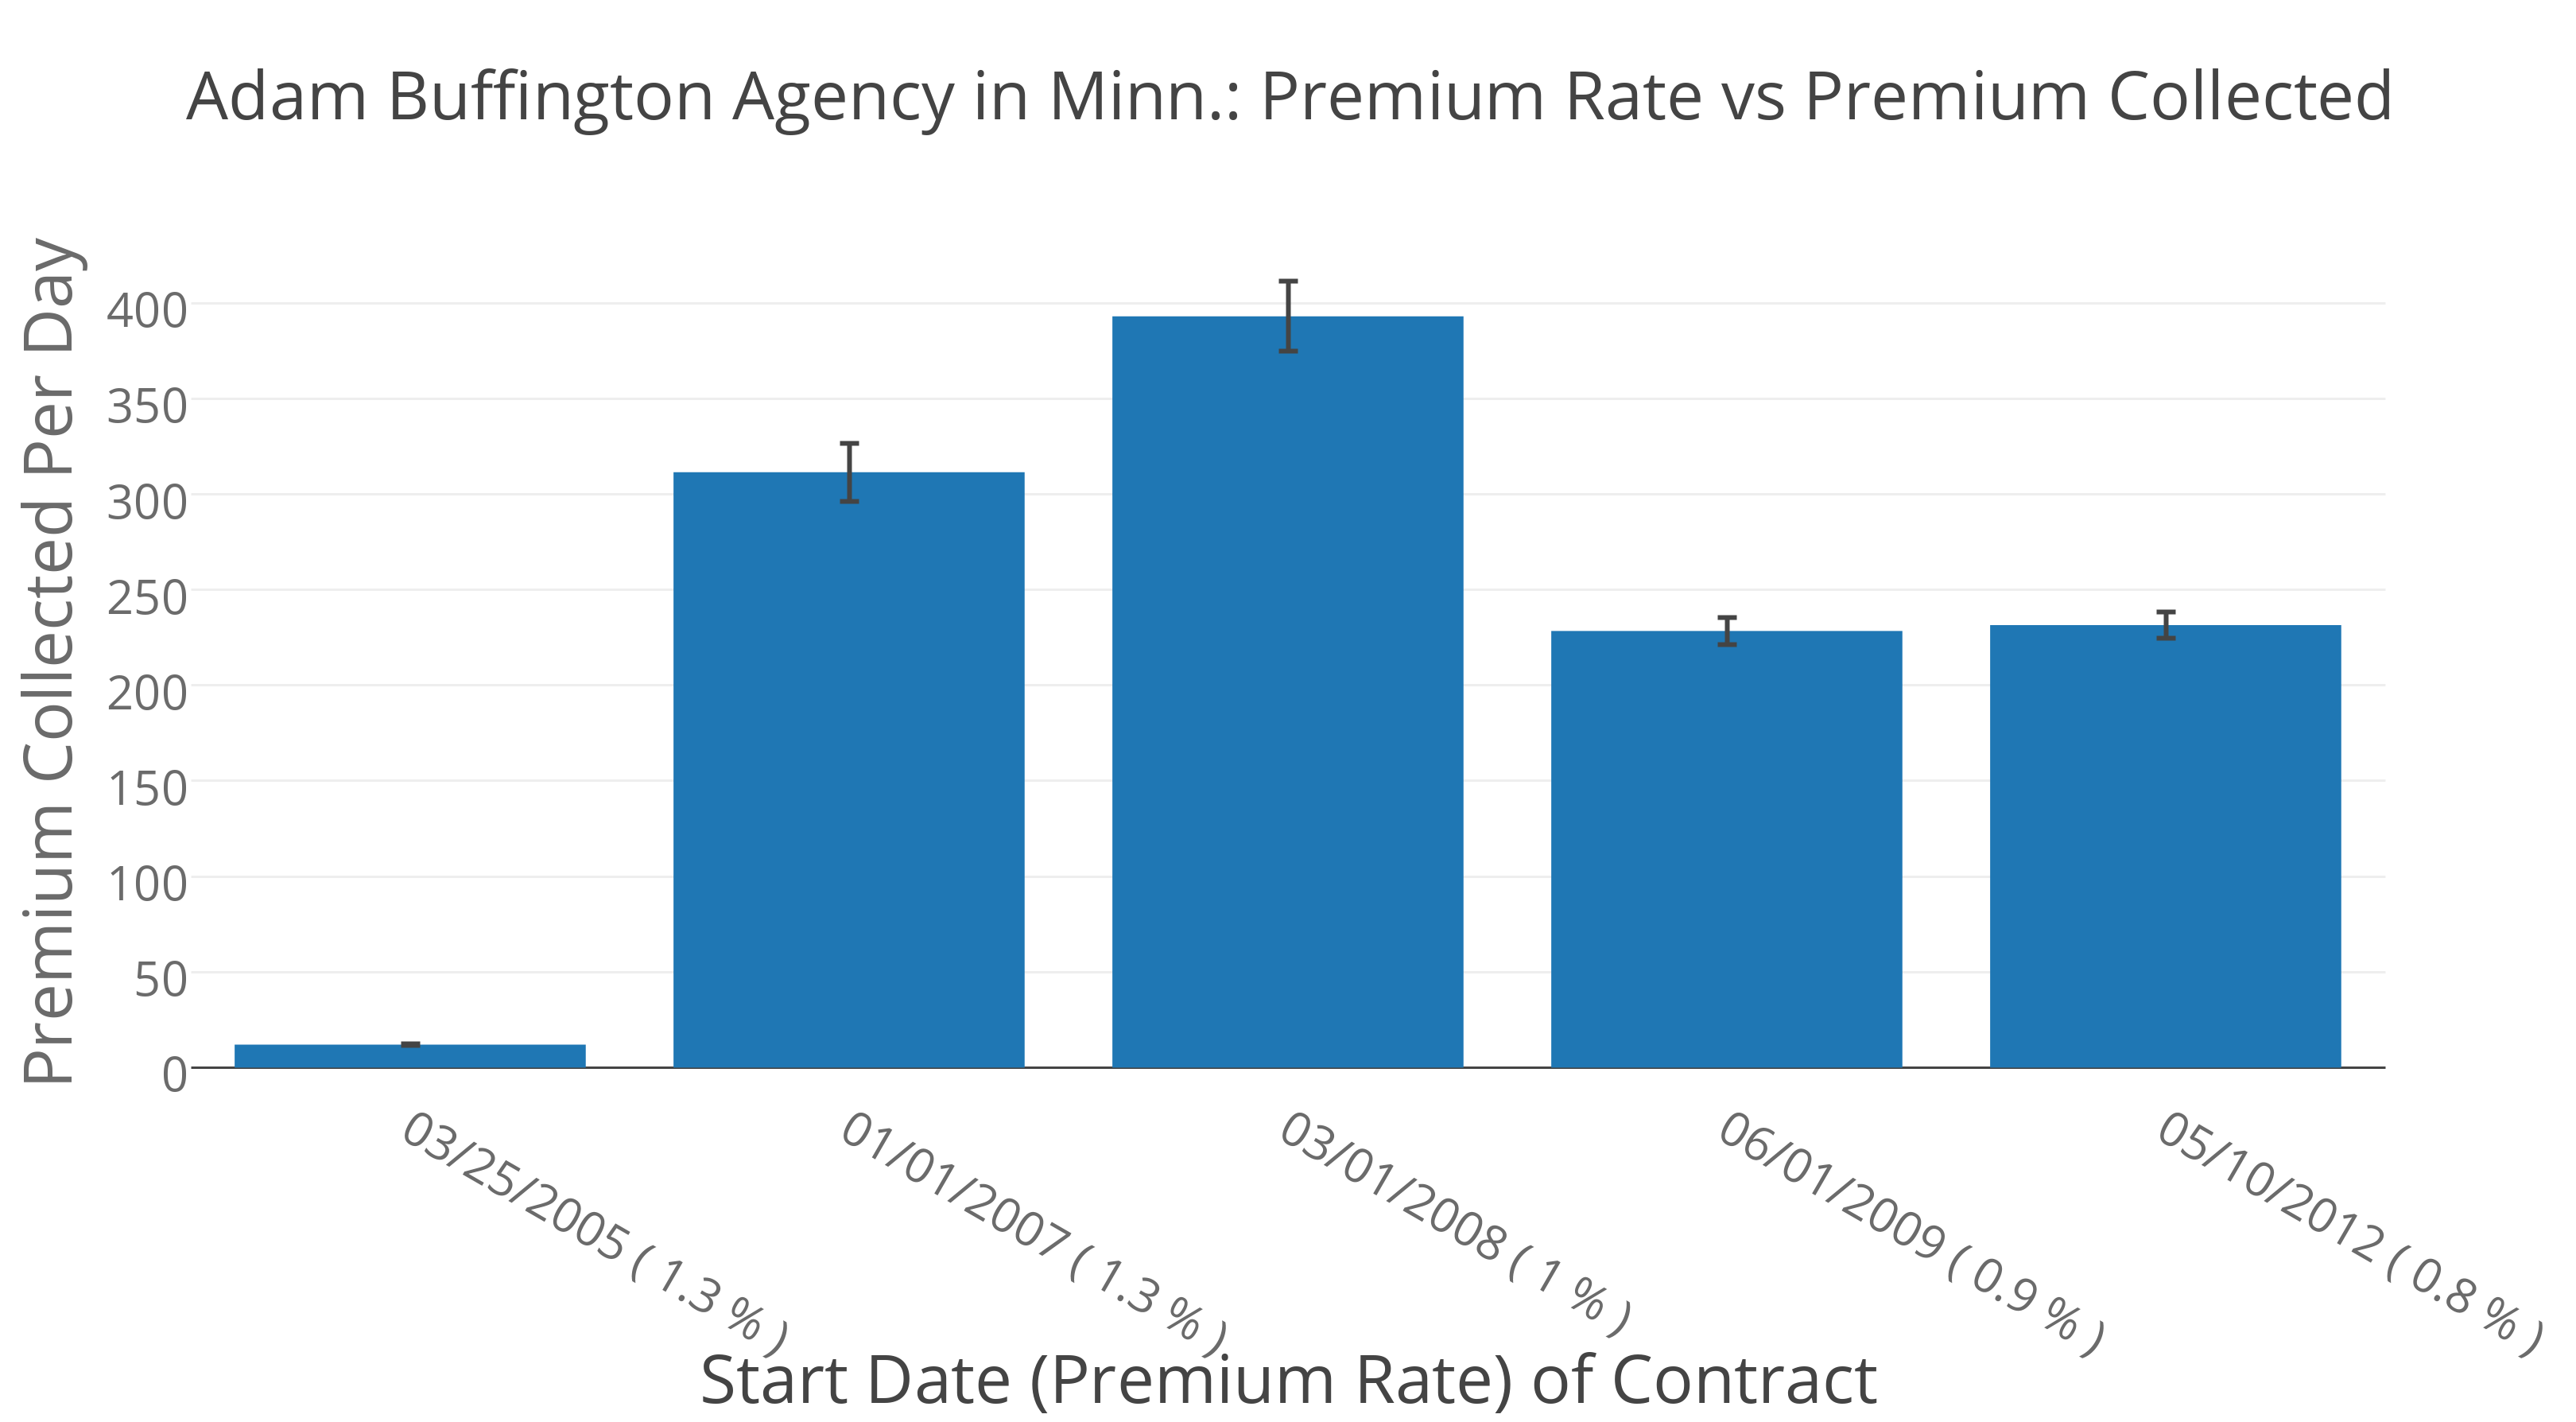
\includegraphics[width=0.34\paperwidth]{Adam_Buffington_Agency_in_Minn-_Premium_Rate_vs_Premium_Collected.png}
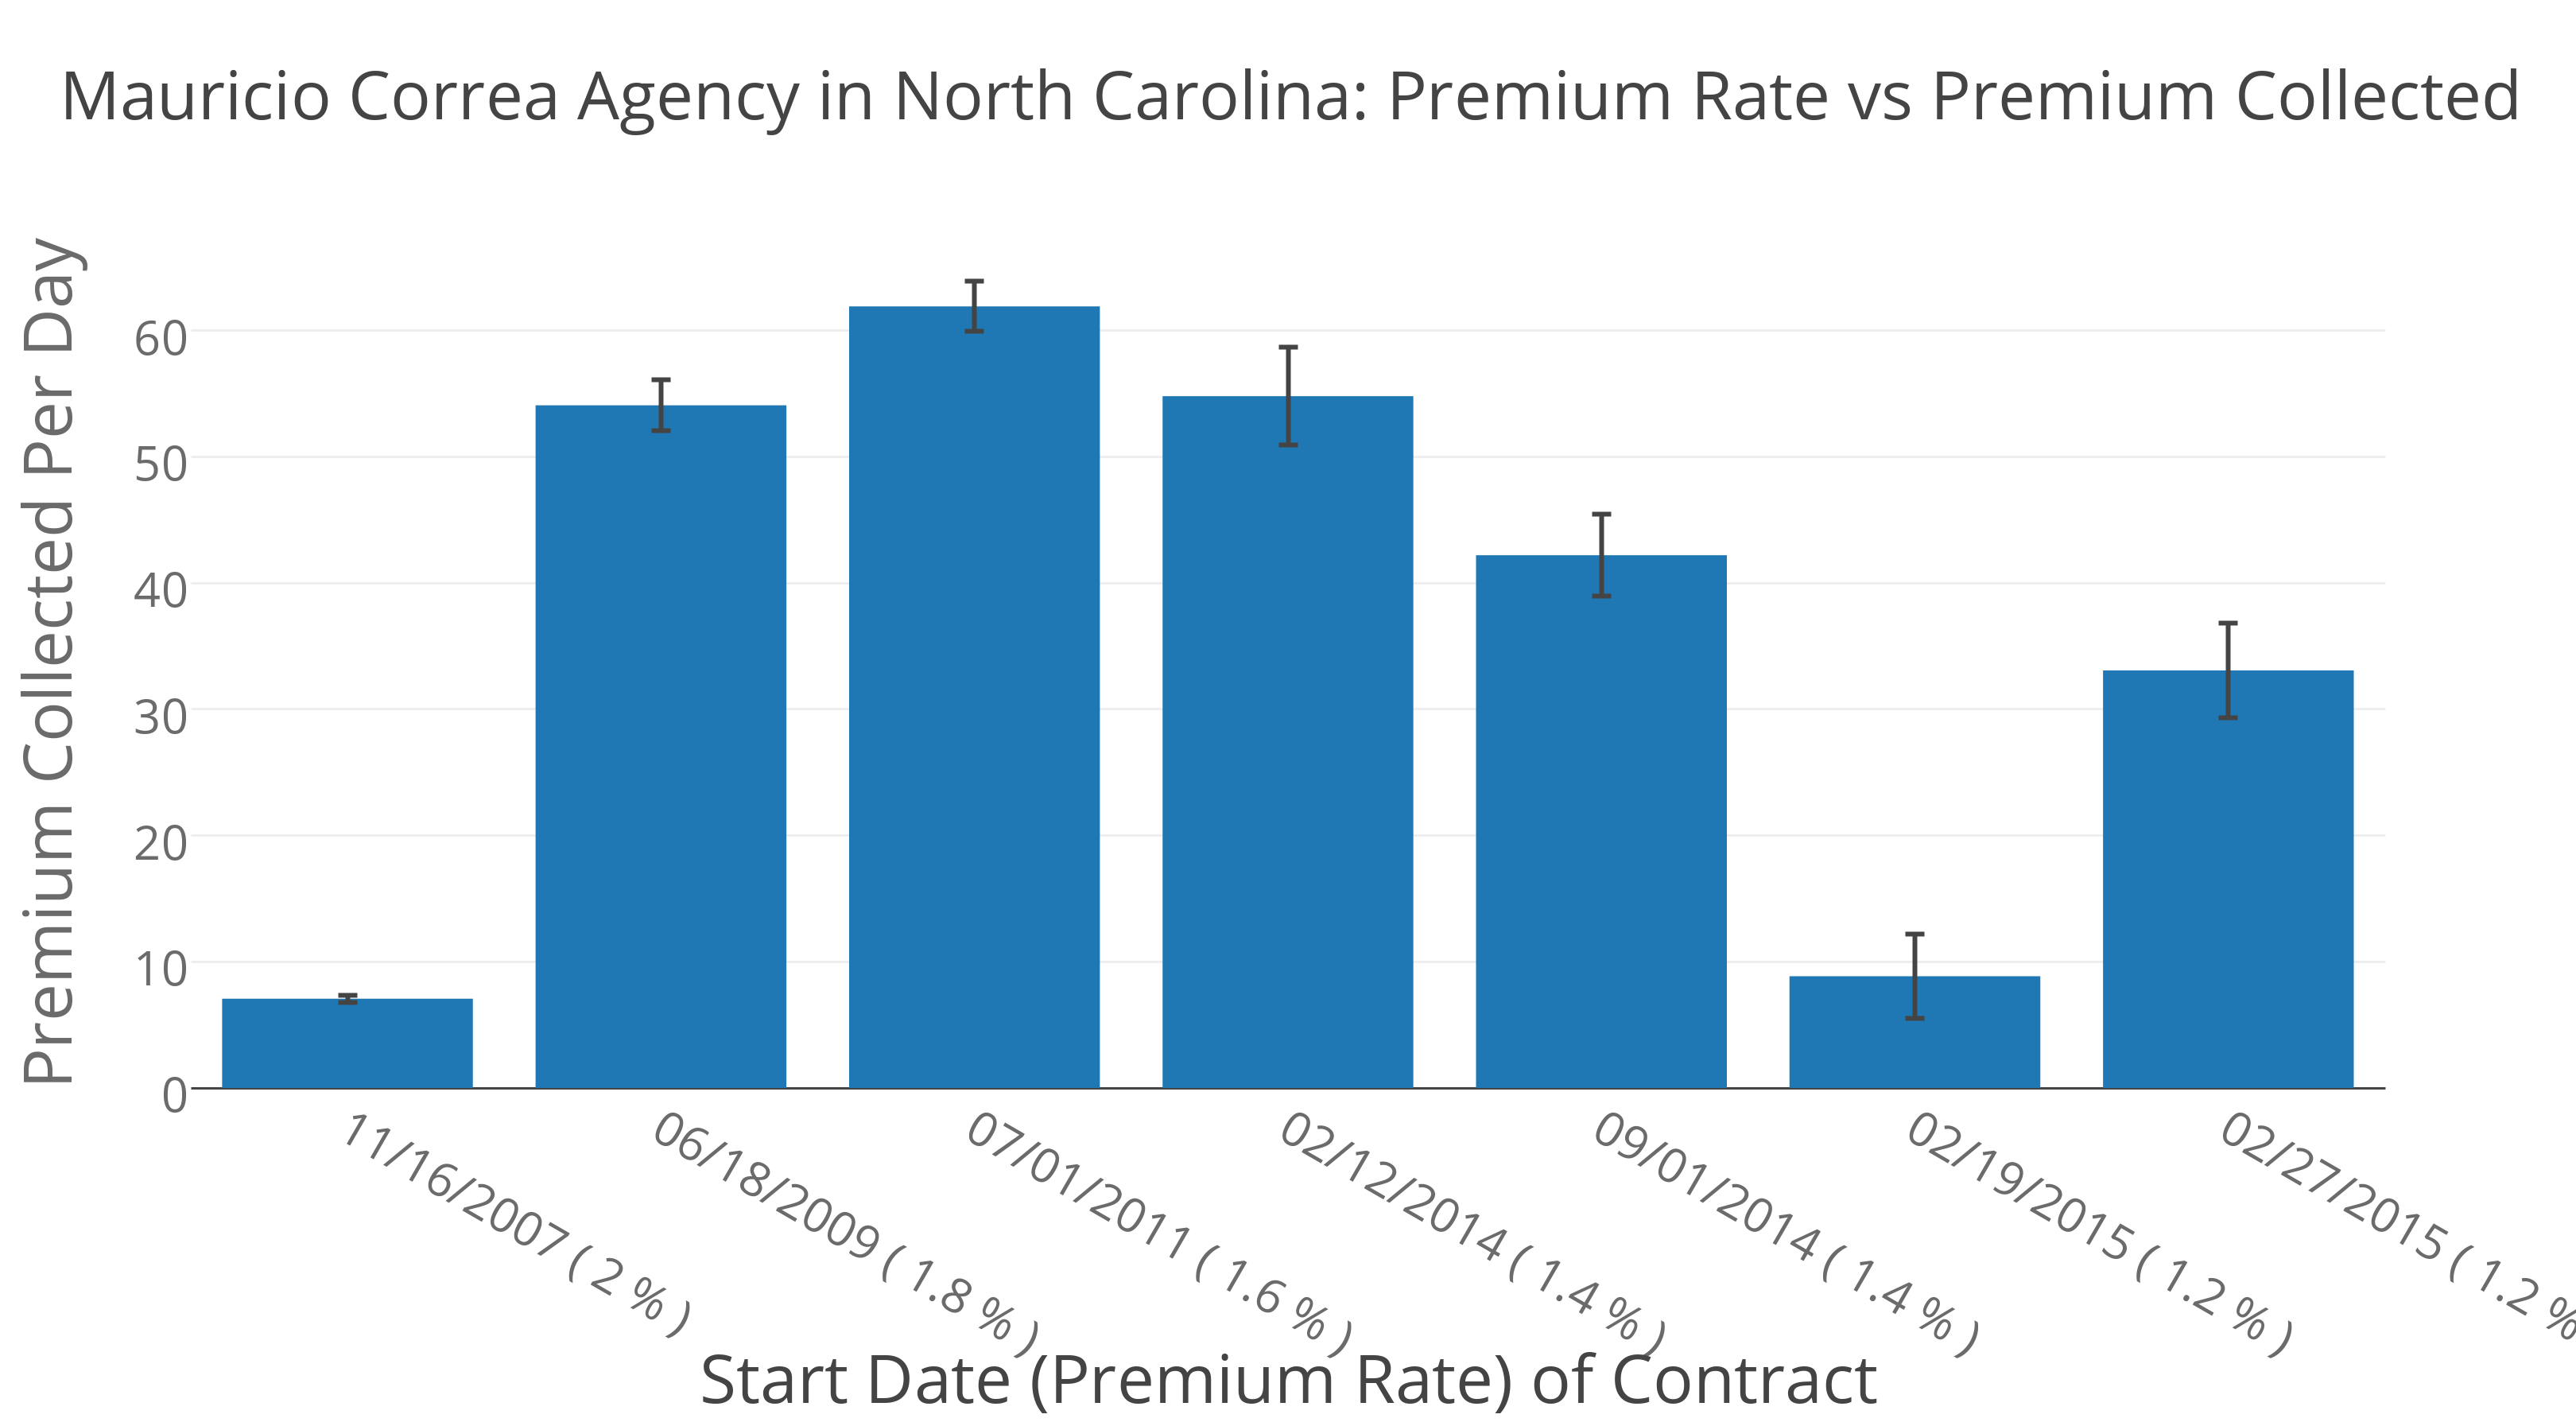
\includegraphics[width=0.34\paperwidth]{Mauricio_Correa_Agency_in_North_Carolina-_Premium_Rate_vs_Premium_Collected.png}
\end{figure}

In some fields, it is entirely expected that your R-squared values will be low. For example, any field that attempts to predict human behavior, such as psychology, typically has R-squared values lower than 50\%. Humans are simply harder to predict than, say, physical processes.


\begin{figure}[b]
\centering
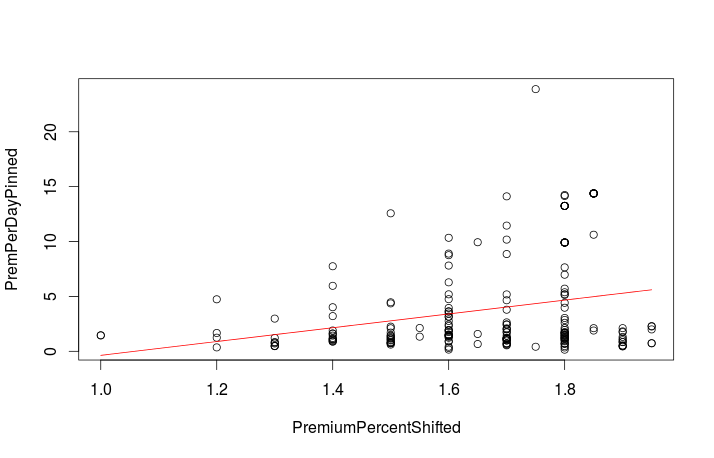
\includegraphics[width=0.45\paperwidth]{pinnedPremPerDay.png}
\end{figure}

\begin{verbatim}
Residuals:
   Min     1Q Median     3Q    Max 
-4.875 -2.978 -1.478  1.250 19.538 

Coefficients:
                      Estimate Std. Error t value Pr(>|t|)    
(Intercept)             -6.677      2.694  -2.478  0.01406 *  
PremiumPercentShifted    6.299      1.613   3.905  0.00013 ***
---
Signif. codes:  0 ‘***’ 0.001 ‘**’ 0.01 ‘*’ 0.05 ‘.’ 0.1 ‘ ’ 1

Residual standard error: 4.266 on 197 degrees of freedom
Multiple R-squared:  0.07183,Adjusted R-squared:  0.06712 
F-statistic: 15.25 on 1 and 197 DF,  p-value: 0.0001296
\end{verbatim}

Adding another variable...\\

\begin{center}
\begin{verbatim}
Residuals:
   Min     1Q Median     3Q    Max 
-5.875 -2.808 -1.090  1.548 20.339 

Coefficients:
                        Estimate Std. Error t value Pr(>|t|)    
(Intercept)           -4.885e+00  2.634e+00  -1.854   0.0652 .  
UnderWritingLimit      1.253e-05  3.118e-06   4.020  8.3e-05 ***
PremiumPercentShifted  4.102e+00  1.648e+00   2.489   0.0136 *  
---
Signif. codes:  0 ‘***’ 0.001 ‘**’ 0.01 ‘*’ 0.05 ‘.’ 0.1 ‘ ’ 1

Residual standard error: 4.111 on 196 degrees of freedom
Multiple R-squared:  0.1425,Adjusted R-squared:  0.1338 
F-statistic: 16.29 on 2 and 196 DF,  p-value: 2.856e-07
\end{verbatim}
\end{center}

\begin{figure}[b]
\centering
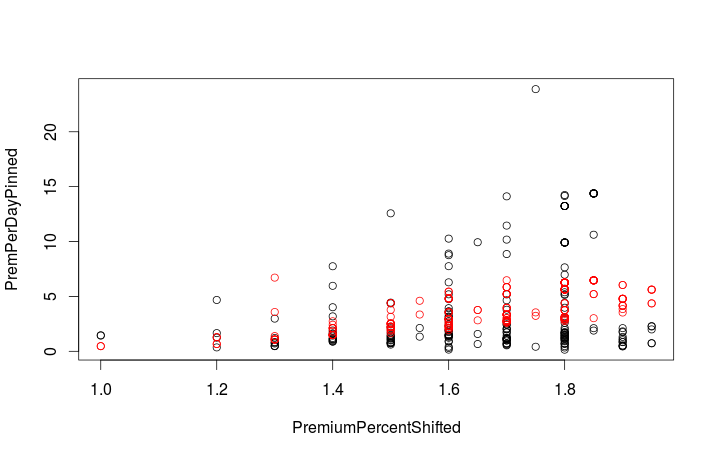
\includegraphics[width=0.45\paperwidth]{pinnedPremPerDayWithUWL.png}
\end{figure}


\end{document}

